\chapter{Grundlagen}

\section{Künstliche Neuronale Netze}

\noindent Bevor wir uns GANs genauer anschauen können, ist es wichtig, die Grundlagen von künstlichen neuronalen Netzen zu verstehen, auf welchen die Technologie fußt.\\

\noindent \acp{KNN} sind ein wichtiger Zweig der Künstlichen Intelligenz und bilden die Basis für Deep Learning-Technologien, welche unter anderem auch GANs umfassen. Sie werden bereits heutzutage erfolgreich in verschiedenen Prozessen, wie Mustererkennung, Kategorisierung- und Prognose von Daten oder Optimierung von Abläufen eingesetzt. Ihre Arbeitsweise liegt darin, eine Menge von Eingaben in sogenannte Eingabevektoren zu kodieren und durch das neuronale Netz daraus eine Menge an Ausgabevektoren zu generieren. Diese Ausgabevektoren können wiederum in ein Ergebnis beliebigen Formats (z.B. Binärdaten, Text, Audio oder Grafiken) kodiert werden. Die Struktur von \acp{KNN} sind von der Funktionsweise des menschlichen Gehirns inspiriert und bestehen aus einer Reihe von miteinander verbundenen Knoten, die als Neuronen bezeichnet werden und als simple Prozessoren fungieren. Diese Prozessoren können nur einfache Operationen ausführen, sind aber in der Lage, komplexe Aufgaben zu erledigen, wenn sie in großer Anzahl miteinander verbunden sind. Die Verbindungen zwischen den Neuronen werden als Kanten bezeichnet und haben ein Gewicht, das die Stärke der Verbindung zwischen den Neuronen angibt. Die Menge der Kanten und deren Gewichtungen definieren dabei die Transformation, welche die Eingangsvektoren beim Durchlauf des \ac{KNN}s erfahren. Die Neuronen sind in Schichten angeordnet, wobei jede Schicht eine Reihe von Neuronen enthält, die eine bestimmte Funktion ausführen. Die erste Schicht wird als Eingabeschicht bezeichnet, die letzte als Ausgabeschicht und alle dazwischen liegenden Schichten werden als versteckte Schichten bezeichnet.\\

\newpage


\begin{figure}[h]
    \centering
    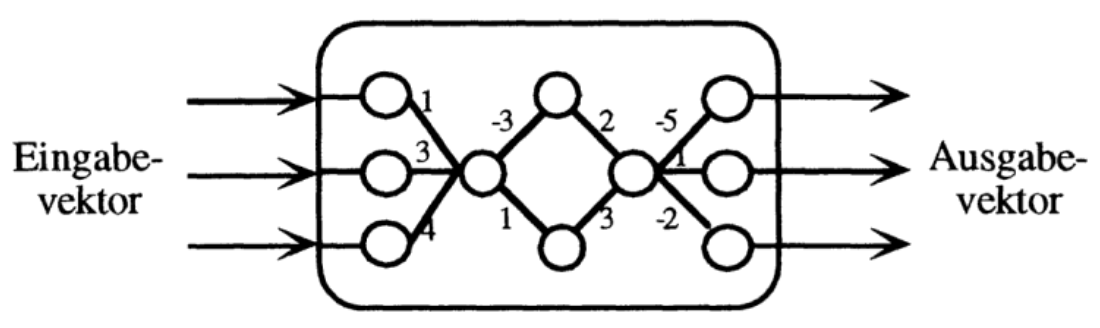
\includegraphics[width=0.50\textwidth]{knn}
    \caption{Schematische Darstellung eines Neuronalen Netzes}
    \label{Abb:basic}
    \end{figure}

%TODO: Vor- und Nachteile

\newpage